\documentclass[a4paper,twoside,linespread=1.5]{ctexrep}

\usepackage[style=utils/caspervector,backend=biber,utf8,sorting=centy]{biblatex}
\usepackage{fancyhdr}%引入页眉页脚宏
\usepackage{array}
\usepackage{graphicx}%图像处理宏
\usepackage{geometry}%页面设置宏
\usepackage{fontspec}
\usepackage{indentfirst}
%\usepackage{setspace}%设置间距宏
\addbibresource{refs/thesis-ref.bib}
\ctexset{
	section/format += \raggedright,
	contentsname = 目 \ 录,
	chapter/fixbeforeskip = true,
	%part/fixbeforeskip = true
}
%设置纸张
\geometry{top=3cm,bottom=2cm,left=2.5cm,right=2.5cm}
%设置默认应为字体
\setmainfont{Times New Roman}
\usepackage[titles]{tocloft}
\renewcommand{\cftdot}{$\cdot$}
\renewcommand{\cftdotsep}{1.5}
\setlength{\cftbeforechapskip}{10pt}

\renewcommand{\cftchapleader}{\cftdotfill{\cftchapdotsep}}
\renewcommand{\cftchapdotsep}{\cftdotsep}

\makeatletter
\renewcommand{\numberline}[1]{%
	\settowidth\@tempdimb{#1\hspace{0.5em}}%
	\ifdim\@tempdima<\@tempdimb%
	\@tempdima=\@tempdimb%
	\fi%
	\hb@xt@\@tempdima{\@cftbsnum #1\@cftasnum\hfil}\@cftasnumb}
\makeatother
\begin{document}
	%页面信息
	%论文题目
\newcommand\thtopic{基于TensorFlow的目标检测与识别}
%学院
\newcommand\academy{信息工程学院}
%专业年级
\newcommand\grade{计算机科学与技术131班}
%作者
\newcommand\thauthor{贺文静}
%指导老师
\newcommand\thtutor{何进荣}
%合作老师
\newcommand\cootutor{}
%完成日期
\newcommand\fishdate{2016年6月}
%学号
\newcommand\sid{2013012982}
%中文摘要内容
\newcommand{\abstractccon}{}
%英文摘要内容
\newcommand{\abstractecon}{}
	%设置页面信息
	\graphicspath{{figures/}}
	
	%封面
	\thispagestyle{empty}
\hfill 学号:\underline{\sid}

\vspace{20mm}

\begin{center}
	
\includegraphics[width=1.7cm,height=1.62cm]{figures/logo.png}
\includegraphics[width=7.82cm,height=1.29cm]{figures/logo2.png}
	\vspace{10mm}
	
	{\songti \huge \hspace{2mm} 2017届本科生毕业论文(设计)}
	
	\vspace{30mm}
	
	{\heiti \huge 题目:\thtopic}
	
	\vspace{30mm}
	
	\begin{table}[h]
		\songti \Large \centering
		\begin{tabular}{lc}
			学院(系):&  \academy\\ 
			\cline{2-2}
			专业年级:&  \grade\\
			\cline{2-2}
			学生姓名:& \thauthor\\
			\cline{2-2}
			指导老师: & \thtutor\\
			\cline{2-2}
			合作指导老师:& \cootutor\\
			\cline{2-2}
			完成日期:&  \fishdate\\
			\cline{2-2}
		\end{tabular}
	\end{table}
\end{center}
	
	%摘要(中英文)
	%% 中文摘要
\chapter*{基于TensorFlow的目标检测与识别}
%\fancypagestyle{plain}{
%\fancyhf{}
%}
\vspace{1em}
{\large {\heiti 摘要: }}\normalsize{\songti 
研究人员每天都收集到海量的基因组数据,有效的查看数据就显得十分重要。基因组可视化 属于 “数据可视化”的一种,相当于数据可视化理论方法在基因组学数据上的具体应用。由于基因组数据的独特性,因此又有着一些独特的可视化方法产生。GBrowse作为在线基因数据可视化工具,可以对目前已知的绝大部分生物数据进行可视化展示,并且其具有强大的可扩展性,尤其对大规模字符串为主的生物学数据具有非常明显的优势。本文通过对苹果基因及其它蔷薇科物种基因可视化的对比,以更加友好的方式显示给研究人员,从而有助于研究者较为透彻辨析苹果基因组同源物基因序列的差异性和相似性,对基因研究人员有着实际应用价值。
}

{\large {\heiti 关键词:}}\normalsize{;优质教育资源;教育教学质量;重要发布;}
\thispagestyle{empty}
	%% 英文摘要
\thispagestyle{empty}
\chapter*{Research on visualization method of apple genome}

\vspace{1em}

\textbf {\large Abstract: }\normalsize{With the advent of the era of big data, various organisms omics data (such as genome,proteome, etc.) showing a trend of rapid growth. Through preliminary investigation found that a morethorough study and organisms (such as Arabidopsis, yeast, etc.) omics data, compared to Malus'smulti-omics data resources in recent years, was able to open access, the data distribution is morefragmented, lack of a unified and efficient management. In order to solve these problems, the
establishment of a multi-omics malus Management System, Malus's multi-omics data integration of resources and effective management. The system uses Struts2 framework to MySQL database, Apache server, combined with JavaScript, Css, Html, Bootstrap and other languages and technology, (1) to achieve a malic 95,232 genes and 95,232 protein sequences, delete, query , modify the basic operation;(2) the use of BLAST sequence alignment tool, Malus realized gene and protein sequence similarity
comparisons and screening; (3) in order to better understand the apple gene or protein function, the
system also provides Arabidopsis Malus similarity search function in gene and protein sequences aspects
of visualization in the genome-wide similarity metric, the site provides links to functional annotation to
help users of the system by means of research more thorough gene or protein function in Arabidopsis,
reasoning apple corresponding homologous gene or protein function. The Malus species researchers have
some practical value}

\textbf{\large Keywords: }\normalsize{Management System; Struts Framework; Apple Multiple Omics; Sequence Alignment}
\thispagestyle{empty}

	
	%设置页脚为罗马字体
	\pagenumbering{Roman}
	
	\tableofcontents
	
	%设置目录页样式(第二页)
	\fancypagestyle{plain}{
		\fancyhf{}
		\fancyfoot[C]{ \thepage}
		\renewcommand{\headrulewidth}{0pt}
		\renewcommand{\footrulewidth}{0pt}
	}
	\thispagestyle{plain}
	
	\clearpage
	
	%\设置页眉样式
	\pagestyle{fancy}
	\fancyhf{}
	\fancyhead[CE]{\thtopic}
	\fancyhead[CO]{\leftmark}
	\fancyfoot[C]{-\thepage-}
	
	%自定义页面样式
	\fancypagestyle{plain}{
		\fancyhf{}
		\fancyhead[CE]{\thtopic}
		\fancyhead[CO]{\leftmark}
		\fancyfoot[C]{-\thepage-}
	}

	%设置正文页面
	\pagenumbering{arabic}
	%绪论
	\chapter{绪论}
\chaptermark{绪论}
	\section{研究背景}

	\subsection{人工智能的发展}
无孔不入的人工智能,别应用在各个领域,比如谷歌传统的搜索和广告业务、无人驾驶汽车,以及医疗健康部门,苹果Siri:为你解决问题的人工智能,应用了人工智能的百度外卖,代替人工顾问的智能应用,作为医疗辅助等。从互联网巨头到初创企业,都将人工智能作为发展的核心,如果关注这方面的新闻,应该看到过这样的一些新闻,"百度以近12亿元剥离游戏业务","央行成立金融科技委员会:用人工智能、云计算丰富监管手段",”苹果斥资2亿美元收购人工智能公司Lattice“等。人工智能变得越来越重要,两会期间,讯飞科大的语音识别及人工智能产品展示时,赢得了一众喝彩。 人工智能不仅涉及到民用,也涉及国家各个核心战略领域。国家主席习近平“一带一路“中演讲。他表示,“一带一路”建设要坚持创新驱动发展,加强在数字经济、人工智能、纳米技术、量子计算机等前沿领域的合作,推动大数据、云计算、智慧城市建设,连接成二十一世纪的数字丝绸之路。在这个人工智能到来的时代,发展人工智能变得越发重要。无论在国内国外,人工智能的发展都被寄予厚望。
	

		\subsection{深度学习的走红}
	随着人工智能的迅速走红,深度学习一词也迅速走红。人工智能是应用范畴的词汇,机器学习是一种实现人工智能的方法,深度学习是一种实现机器学习的方法,也是现有机器学习方法中,最奏效的一类。三者的关系见图1-1,人工智能是最外面的,下来是机器学习,最里面的是深度学习。而计算机视觉是机器学习应用最成功的一个方面,发展最为迅猛的一个分支。计算机视觉在很多方面都有应用,最为大家熟知的有人脸识别,组织恶意软件,语音识别,	无人驾驶汽车,在生物,医学方面也都有一定的应用,实际上,思科的一个评估显示,在2016年互联网上超过85\%的信息都会是像素形式,我们进入“多媒体”时代,视觉的时代,图片和视频的时代。由于互联网作为信息的载体,以及大量(视觉)传感器引发了视觉信息的大爆炸。CS231a深度学习与计算机视觉课程开篇,李菲菲教授讲计算机视觉(CV)她将这些视觉信息称为“互联网中的暗物质”,并且举了YouTube的一个例子,我们没法对这么大量的数据进行浏览,标记,分类,索引等,但是使用计算机视觉技术能够对照片进行标签、分类、处理视频中的每一帧,自动截取出篮球比赛中----比如说科比的一次精彩进球,我们现在面临着的问题就是,大量的数据,以及这些“暗物质”的挑战。目标识别与检测作为计算机视觉的一个应用,是很有应用价值的问题,而且是很多问题的根本解决之策。
	
		\subsection{TensorFlow的出现}	
	2015年11月,谷歌宣布TensorFlow开源,由于其灵活的架构可以在一个或多个CPU,GPU、桌面、服务器、以及移动设备上部署,还不用重新编写代码,其分布式计算的方法大大缩短了机器学习的训练时间,核心代码是C++编写的简化了线上部署的复杂度,还有Python、GO、Java的接口,用户可以很容易的使用,可视化的TensorBoard,极快的编译速度,并行计算模式等优点,使其作为一个开源软件库,刚开源第一个月就积累了10000+的star,而到现在star数已经到了56939, 是GitHub上最受欢迎的深度学习框架。在图形分类、音频处理、推荐系统和自然语言处理等场景下都有丰富的应用。最近流行的Keras框架底层默认使用TensorFlow,著名的斯坦福CS231n课程使用TensorFlow作为授课和作业的编程语言,而且现在除了谷歌内部大规模使用之外,优步(Uber)、Twitter、京东、小米、FaceBook等都在使用。TensorFlow的contrib.learn模块提供了一个让开发人员从scikit-learn或Keras进入到TensorFlow的桥梁,避免了从一个框架转移到另一个框架的无措感。TensorFlow的出现使更多对机器学习感兴趣的人可以去涉足这个领域,而不是因为电脑硬件的问题,机器学习训练时间过长的问题驻足。
	人工智能,机器学习,深度学习,TensorFlow成为越来越受欢迎的话题,我在百度指数,以及Google trends上,分别输入了机器学习,深度学习,还有人工智能几个搜索词后,得到的搜索热度趋势图见图1-2。通过这些数据得出的结论是人工智能,深度学习,正在变得越来重要,正在引起越来越多的重视。而在Google trends中看到TensorFlow搜索热度趋势图见图1-3 。TensorFlow的热度基本维持在100,足以说明这是目前很受欢迎的一个话题。
		\begin{figure}[p]
		\centering
		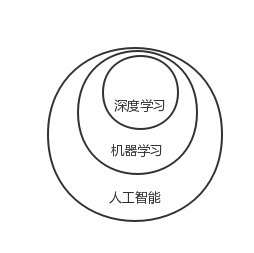
\includegraphics[width=0.7\linewidth]{figures/1-1}
		\caption[人工智能,机器学习,深度学习三者的关系图]{}
		\caption{}
		\label{fig:1-1}
	\end{figure}
	\begin{figure}[p]
		\centering
		
\includegraphics[width=0.5\linewidth]{figures/1-2}
		\caption{Google trends搜索热度趋势图:词汇的热度按0~100分为100个等级,可以看出来三者都呈上升趋势,并且相当的受欢迎。}
		\label{fig:1-2}
	\end{figure}
	\begin{figure}[p]
	\centering
	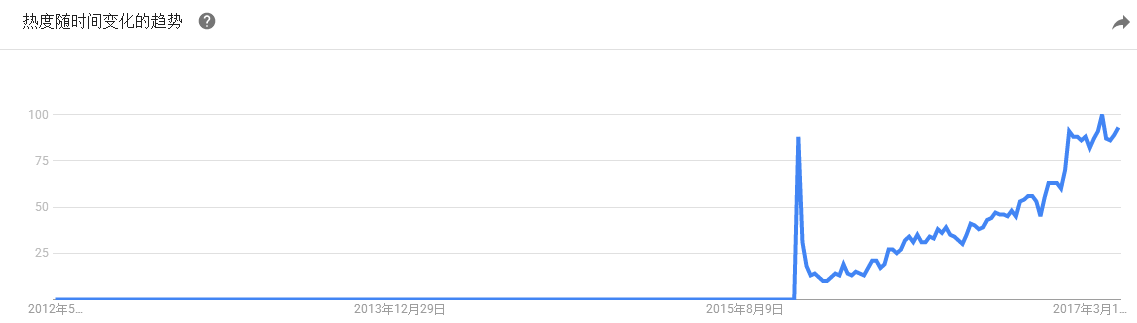
\includegraphics[width=0.5\linewidth]{figures/1-3}
	\caption[TensorFlow 在谷歌搜索的热度趋势]{}
	\caption{}
	\label{fig:1-3}
\end{figure}
\section{深度学习}
\subsection{}

		
	\section{本文研究内容}
		
		
	\section{本文内容安排}
	
	
	%论文主体内容
	\chapter{深度学习平台——TensorFlow}
\chaptermark{深度学习平台——TensorFlow}
	%GBrowse
	\section{TensorFlow简介}
	TensorFlow在2015年11月由Google开放,从此,它已经成为GitHub上最受欢迎的机器学习库。TensorFlow——第二代分布式机器学习算法实现框架和部署系统,是基于使用DisBelief时的经验及训练大规模分布是神经网络的需求开发的。但是在某些基准上,TensorFlow是DistBelief的两倍。可以方便地部署到各种平台,大大简化了真实场景中应用机器学习的难度。TensorFlow的计算可以表示为有状态的数据流式图,使用数据流式图来规划计算流程,可以将计算映射到不同的硬件和操作系统平台。对于大规模的神经网络训练,TensorFlow可以让用户简单地实现并行计算,同时使用不同的硬件资源进行训练,同步或异步地更新全局共享的模型参数和状态。
	TensorFlow是相对高阶的机器学习库,用户可以方便的用它设计神经网络结构,支持自动求导,核心代码是用C++编写的,简化了线上部署的复杂度,可以在手机和CPU这种内存紧张的设备上运行。除了C++接口外还有Python、Go、Java等接口。可以部署在一台或多台CPU、GPU上,兼容多个平台,包括Windows、Linux、Android等。有TF.Learn和TF.Slim等上层组件可以帮助快速的设计新网络,并且兼容Scikit-learn estimator接口,同时TensorFlow不局限于神经网络,数据流式图支持非常自由的算法表达,只要可以将计算表达成计算图的形式,就可以使用TensorFlow。
	另一个重要特点是它灵活的移植性,可以将同一份代码几乎不经过修改就轻松的部署到任意数量CPU或GPU的PC、服务器或者移动设备上。还有一个优势就是极快的编译速度,还有功能强大的TensorBoard,能可视化网络结构和训练过程,对于观察复杂的网络结构和监控长时间、大规模的训练很有帮助。
	\section{核心概念}
		\subsection{计算图}
		计算图是TensorFlow最基本的一个概念,TensorFlow中的所有计算都会被转化为计算图上的节点。TensorFlow中的计算可以表示为一个有向图(directed graph)、数据流图,称为计算图(computation graph) 
		TensorFlow是一个通过计算图的形式来表述计算的编程系统,其中每一个运算操作(operation)将作为一个节点(node),节点与节点之间的连接成为边(edge)。计算图中每一个节点可以有任意多个输入和任意多个输出,节点可以算是运算操作的实列化。在计算图的边中流动(flow)的数据被称为张量(Tensor),这个也是Tensoflow名字的由来。没有数据流动的边被称为依赖控制。计算图描述了张量数据的计算流程,负责维护和更新状态,对分支进行条件控制和循环操作。如果机器上有超过一个可用的 GPU, 除第一个外的其它 GPU 默认是不参与计算的. 为了让 TensorFlow 使用这些 GPU, 你必须将 op 明确指派给它们执行. with...Device 语句用来指派特定的 CPU 或 GPU 执行操作
		\begin{figure}[!ht]
			\centering
			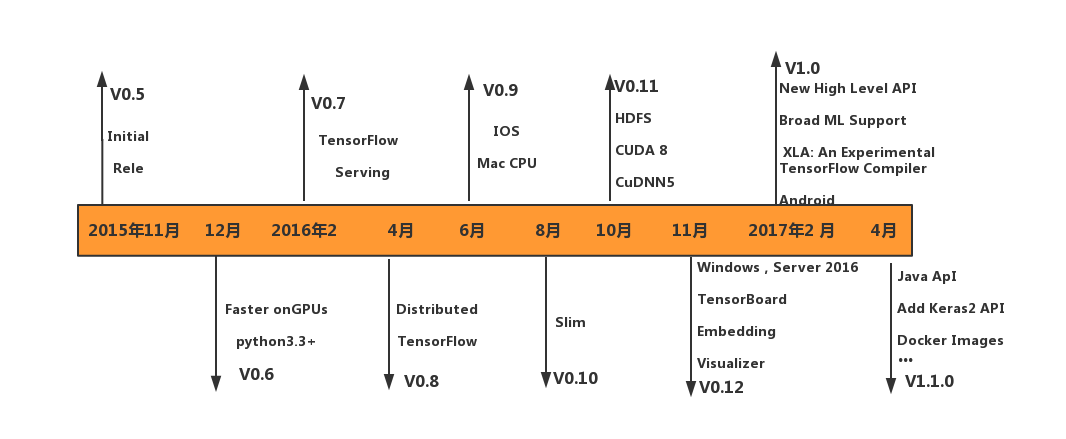
\includegraphics[width=0.5\textwidth]{figures/2-1}
			\caption{计算图示例}
			\label{fig:2-1}
		\end{figure}
		
		\subsection{运行模型}
		Session(会话)是用户使用TensorFlow时的交互式接口。Session拥有并管理TensorFlow程序运行时的所有资源。当所有计算完成之后需要关闭会话来帮助系统回收资源,否则就可能出现资源泄漏的问题。TensorFlow中使用Session的模式一般有两种,第一种模式需要明确调用会话生成函数和关闭会话函数,第二种模式是通过Python的上下文管理器来使用会话,这种模式为了解决异常退出时资源释放的问题,TensorFlow的会话不会自动生成默认的会话,需要手动指定,当默认的会话被指定之后可以通过tf.Tensor.eval()函数计算一个张量的取值,在交互式环境下(比如Python脚本等)通过设置默认会话的方式来获取张量的取值更加方便,函数tf.InteractiveSession()在交互式环境下直接构建默认会话。使用这个函数会自动将生成的会话注册为默认会话。可以省去将产生的会话注册为默认会话的过程,无论哪种方法都可以通过ConfigProto Protocol Buffer 来配置需要生成的会话,通过ConfigProto可以配置类似并行的线程数,GPU分配策略,运算超时时间等参数。在这些参数中最常使用的有两个allow\_soft\_placement=和log\_device\_placement都是布尔型的参数。 
		在实现上, TensorFlow 将图形定义转换成分布式执行的操作, 以充分利用可用的计算资源(如 CPU 或 GPU)。 一般你不需要显式指定使用 CPU 还是 GPU, TensorFlow 能自动检测。如果检测到 GPU, TensorFlow 会尽可能地利用找到的第一个 GPU 来执行操作。
		
		\subsection{数据模型}
		张量是TensorFlow管理数据的形式,可以被简单的理解为多维数组。其中零阶张量表示标量(scalar),也就是一个数;第一阶张量为向量(vector),也就是一个一维数组;第n阶张量可以理解为一个n维数组。在张量中并没有真正保存数字,它保存的是如何得到这些数字的计算过程。TensorFlow计算结果不是一个具体的数字,而是一个张量的结构,一个张量主要有三个属性:名字(name),维度(shape),类型(type) 
		第一个属性名字不仅是一个张量的唯一标识符,还给出了这个张量是如何计算出来的,张量和计算图上节点所代表的计算结果是对应的,张量的命名可以通过“node:src\_output”的形式给出,其中node为节点的名称,src\_output表示当前张量来自节点的第几个输出。 
		第二个属性是张量的维度(shape)描述了一个张量的维度信息。 
		第三个属性是类型(type)每一个张量会有一个唯一的类型,TensorFlow会对参与运算的所有张量进行类型检查,当发现类型不匹配时会报错。 
		TensorFlow支持多种不同的类型,主要包括了实数(tf.float16 tf.float32,tf.float64)、整数(tf.int16,tf.int32,tf.int64,tf.int8,tf.uint16,tf.uint8)、布尔型(tf.bool),复数型(tf.complex64,tf.complex128)等。 对于张量的使用,可以分为两大类。第一类是对中间计算结果的引用。当一个九三包含很多中间结果时,使用张量可以大大提高代码的可读性。第二类是当计算图构造完成之后,张量可以用来获得计算结果,结合会话使用tf.Session().run(result)就可以得到真实的数字.
		\subsection{变量}
		在TensorFlow中,变量的作用就是保存和更新神经网络的参数。变量包含张量 (Tensor)存放于内存的缓存区。建模时它们需要被明确地初始化,模型训练后它们必须被存储到磁盘。这些变量的值可在之后模型训练和分析是被加载。 TensorFlow提供了一个通过变量名来创建或者获取一个变量的机制。通过这个机制,在不同的函数中可以直接通过变量的名字来使用变量,而不需要将变量通过参数的形式到处传递,这个机制主要通过tf.get\_variable()和tf.variable\_scope()函数实现的。
	\section{Tensorflow环境搭建}
	Tensorflow对各种主流的操作系统的支持都比较完善,本文将使用Tensorflow对Python提供的API进行研究学习。Tensorflow支持的Python环境有Python2.7和Python3.5,目前最新版本的Tensorflow支持Python3.5。Tensorflow环境的搭建可以分为两类,第一种是使用官方提供的发行进行安装使用,第二种是下载Tensorflow的源代码进行编译安装使用。本小节将以第一种方式在Linux和Windows系统环境下分别使用Pip和Anaconda进行环境搭建。
		\subsection{Pip下环境搭建}
		Pip是一个安装,管理Python软件包的工具,通过Pip可以安装已经打包好的TensorFlow以及TensorFlow所需要的依赖关系。环境需保证操作系统上有Python的环境,首先,安装Python的Pip包,然后通过Pip命令针对不同版本的Python安装CPU或者GPU版本的Tensorflow。如下安装过程的详细代码。
		\begin{lstlisting}
		 sudo apt-get install python-pip python-dev
		 pip install tensorflow  # Python 2.7; CPU support (no GPU support)
		 pip3 install tensorflow # Python 3.n; CPU support (no GPU support)
		 pip install tensorflow-gpu  # Python 2.7;  GPU support
		 pip3 install tensorflow-gpu # Python 3.n; GPU support
		\end{lstlisting}
		\subsection{Anaconda下环境搭建}
		Anaconda是由Python开发的领先的开放数据科学平台。 包括超过100种最受欢迎的数据科学Python,R和Scala软件包。内置了数百个Python经常用的库,包括Scikit-learn、Numpy、SciPy、Pandas等。 首先,需要安装Anaconda的环境,其次创建Python不同版本的环境,最后通过pip安装TensorFlow的环境。如下安装过程的详细代码。图2-2安装成功后测试图。
		\begin{lstlisting}
		Anaconda3-4.3.1-Windows-x86_64.exe #Windows Install
		bash Anaconda3-4.3.1-Linux-x86_64.sh #Linux Install
		conda create --name python35 python=3.5 # create environment in Linux and Windows
		source activate Python35 # Linux
		activate Python35 #Windows
		pip install tensorflow #install TensorFlow
		\end{lstlisting}
		
		\begin{figure}[!ht]
			\centering
			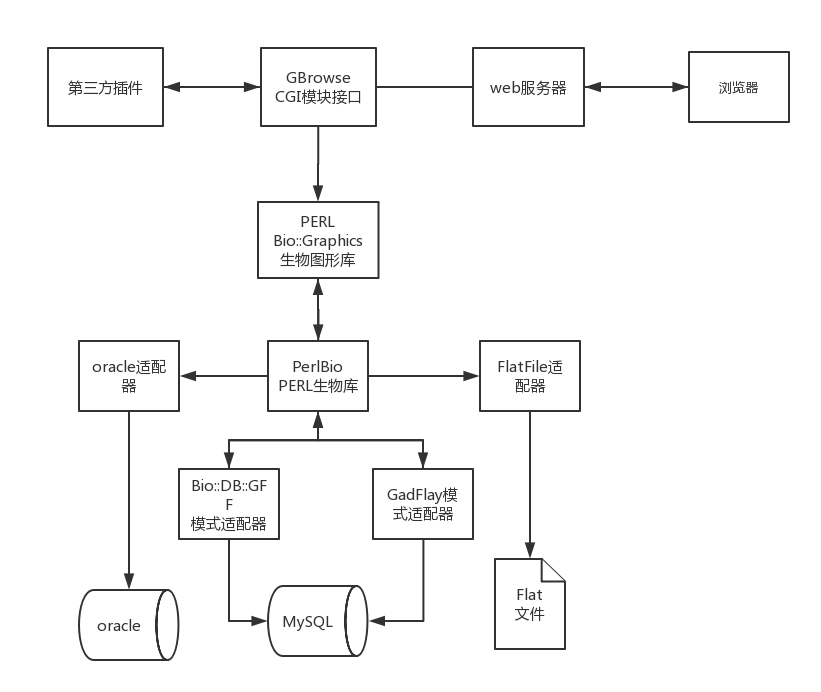
\includegraphics[width=0.8\textwidth]{figures/2-2}
			\caption{TensorFlow安装成功}
			\label{fig:2-2}
		\end{figure}
	\chapter{基因组浏览器环境搭建与配置}
	\chaptermark{基因组浏览器环境搭建与配置}
	\section{GBrowse搭建与配置}
	\subsection{操作系统安装与配置}
	\subsection{源码安装Apache与MySQL}
	\subsection{GBrowse全局配置文件编写}
	\subsection{GBrowse苹果基因组配置文件编写}
	\subsection{全局配置Apache与GBrowse进行模块关联}
	\subsection{全局配置MySQL与GBrowse进行模块关联}
	\section{JBrowse搭建与配置}
	\section{UCSC Genome Browser搭建与配置}
	\chapter{数据的处理与导入}
	\chaptermark{数据的导入与处理}
	\section{系统要求}
	\section{数据转储}
	\chapter{苹果基因与蔷薇科植物基因可视化对比验证}
	\chaptermark{苹果基因与蔷薇科植物基因可视化对比验证}
	\section{拟南芥基因可视化}
	\section{红桃基因可视化}
	\section{验证实验结果}
	\chapter{总结与展望}
	\chaptermark{总结与展望}
	\section{总结}
	\section{展望}
	\newpage
	%参考文献
	\addcontentsline{toc}{chapter}{参考文献}
\nocite{*}
\printbibliography[title=参考文献]
\fancypagestyle{plain}{
	\fancyhf{}
	\fancyhead[CE]{参考文献}
	\fancyhead[CO]{参考文献}
	\fancyfoot[C]{-\thepage-}
}
	%致谢
	\chapter*{致谢}
\addcontentsline{toc}{chapter}{致谢}

时间如白驹过隙,四年的大学生活转眼就结束了。

在这短短的四年里,经历了许许
多多的事情,有快乐有悲伤,也曾遇到挫折也曾彷徨,好在身旁有许许多多帮助我的人,
首先感谢我的导师于建涛老师, 于老师工作十分负责,非常关注我的毕业设计进度
并且在遇到困难的时候给予我思路和方向, 于老师严谨细致的工作作风一直伴随着我整
个毕业设计的过程,时刻激励着我对整个毕业设计的改进和优化。在此, 我非常感谢于
老师对我的毕业设计和论文的帮助和支持。

感谢我的舍友们,在这四年里是你们一直陪伴在我的身边,在我遇到困难的时候伸
出援手帮助我度过难关。

感谢我的爸爸妈妈, 无论什么时候都爸爸妈妈在背后默默支持我、鼓励我,让我顺
利的完成了学业,并将继续支持我出国深造,是你们的支持给予了我前进的动力, 让我
有力量继续走下去。

现在论文即将完成,心情很是激动,回想起从一开始的选题到现在论文的完成,我
经历了许许多多,在这期间也有许许多多的人给予我无私的帮助,在此请接受我最诚挚
的感谢。

\fancypagestyle{plain}{
	\fancyhf{}
	\fancyhead[CE]{致谢}
	\fancyhead[CO]{致谢}
	\fancyfoot[C]{-\thepage-}
}
\end{document}